\clearpage
\section{The build}

\begin{figure}[H]
	\centering
	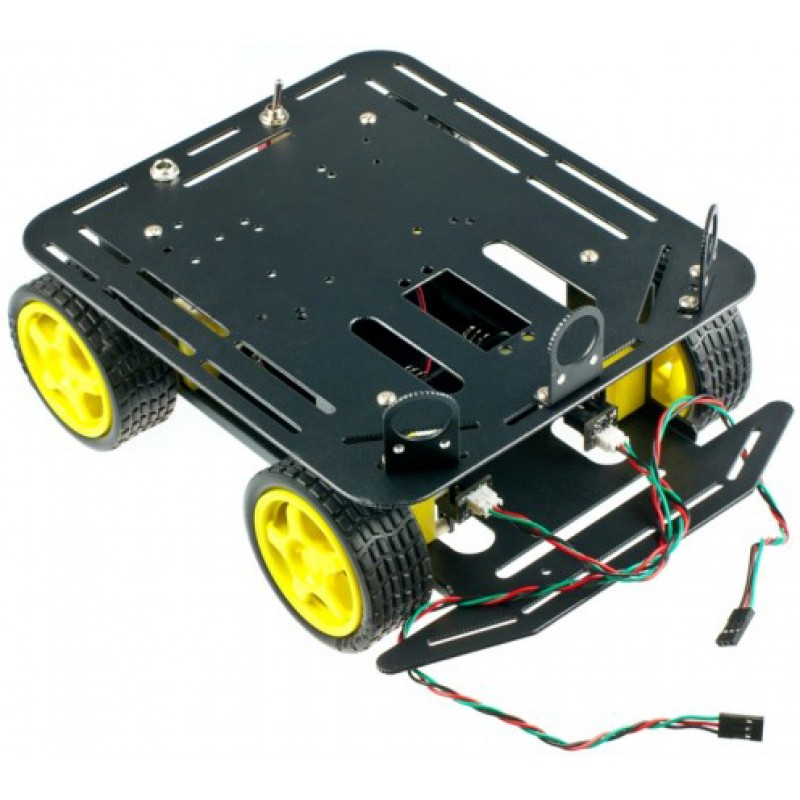
\includegraphics[width=.4\linewidth]{images/chassis.jpg}
\end{figure}
%Write about choice of chasis

To attach the different sensors to the rover, different enclosures and brackets were needed. For the ultrasonic sensors, two different kind of brackets have been designed, since the main chassis required them to be mounted differently based on their placement on each of the four sides. Using Autodesk Inventor the two enclosures for the ultrasonic sensors have been modelled and 3d-printed.

\begin{figure}[H]
	\centering
	\begin{subfigure}[H]{0.4\textwidth}
		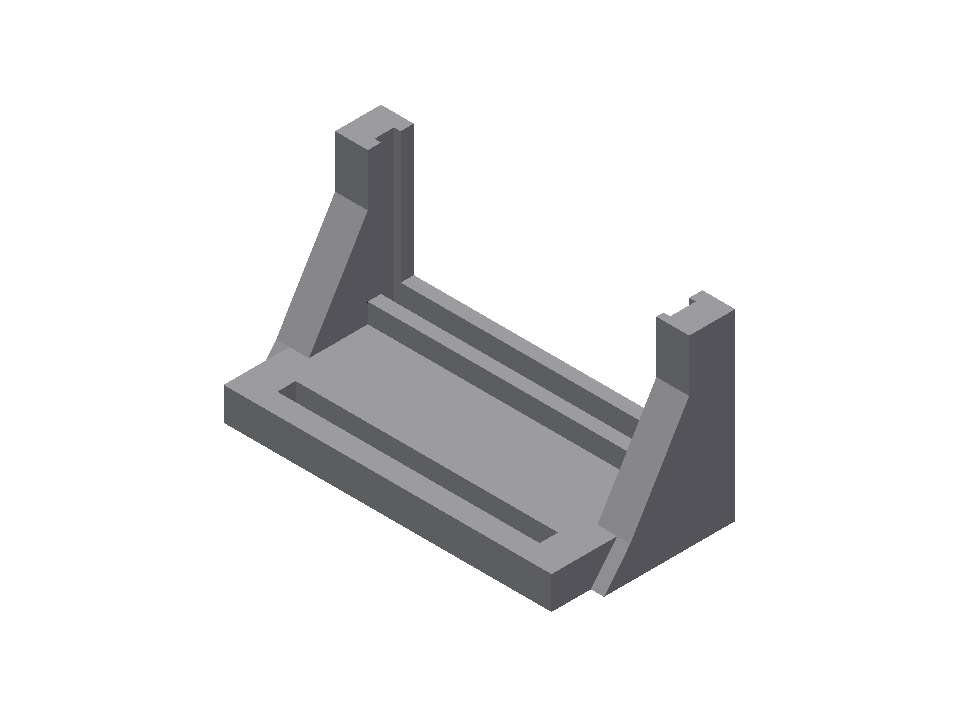
\includegraphics[width=\textwidth]{images/ultrasonicholder.jpg}
	\end{subfigure}%
	\quad
	\begin{subfigure}[H]{0.4\textwidth}
		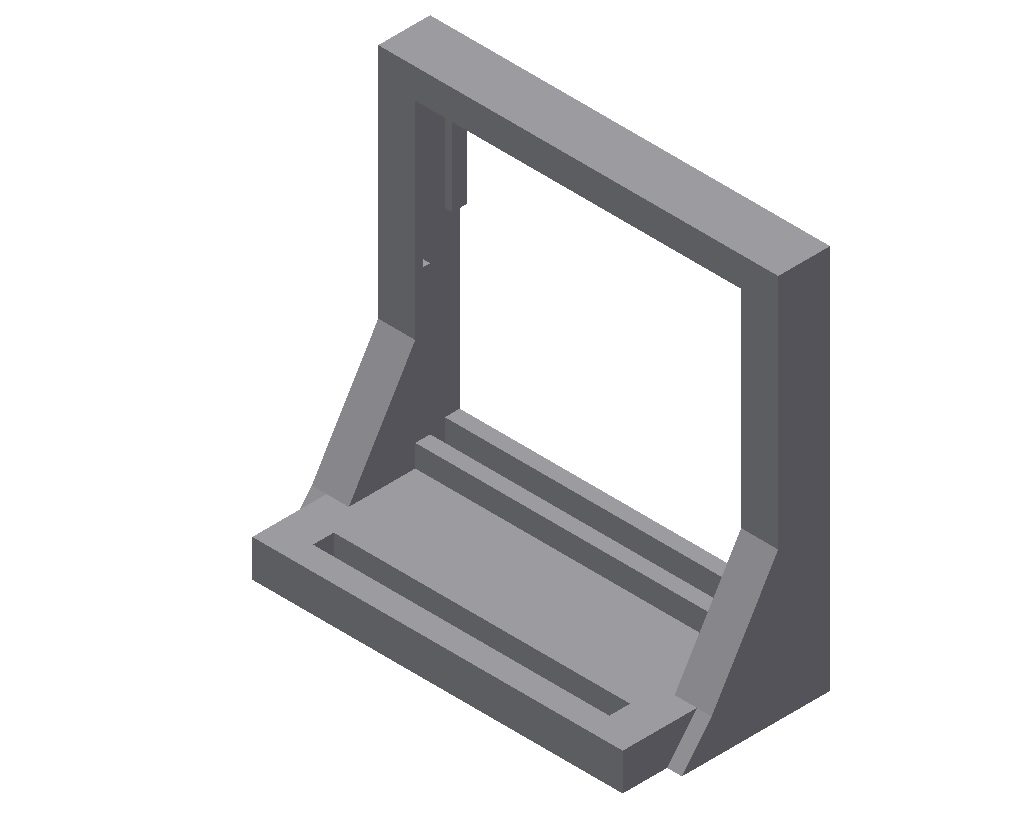
\includegraphics[width=\textwidth]{images/ultrasonicholder-upsidedown.jpg}
	\end{subfigure}
	\caption{The enclosures used to mount the ultrasonic sensors on the chassis}
\end{figure}

The enclosures for the ultrasonic sensors have be designed to place all of the sensors at the same height on each side of the chassis, to ensure that the measurements are similar.

%Add pictures of the mounted sensors

The design for the Lidar enclosure was found on the internet, which was already made by someone who had created a similar project. The reasoning behind using that specific design is that flawlessly allows the Lidar to rotate 360degrees using the same components.\cite{lidarenclosure}.
%further description of the lidar set-up needed

%Add pictures of the lidar enclosure